\documentclass{article}

\usepackage{graphicx}


\begin{document}


\section{Data mining}

I downloaded the full database of dna-ligand complexes, containing 400 structures. I then filtered it down to ones that are intercalators complexes, resulting in \emph{32} structures. Went through all of them to identify candidate structures that could be simulated (visual inspection). Final result is 12 crystal structures that can consitute as starting points for simlulations.

\section{Protocol}

Based on the BSC1 forcefield paper, I set up the following protocol: energy minimization, 2 ns of restrained equilibration, 1 ns of unrestrained equilibration, production simulation. The length of this is to be determined and depends on the specific free energy protocol.

\section{First test on 1G3X}

As the most plausable structure, I chose 1G3X as the first example to simulate. I was able to parametrise the ligand using the AM1-BCC atomic charge generation method, the GAFF2 force field. The DNA was parametrised with BSC1 forcefield. As benchmark simulation I ran 2 ns on 1 GPU node, with average performace of 90-100 ns/day.

\begin{figure}
  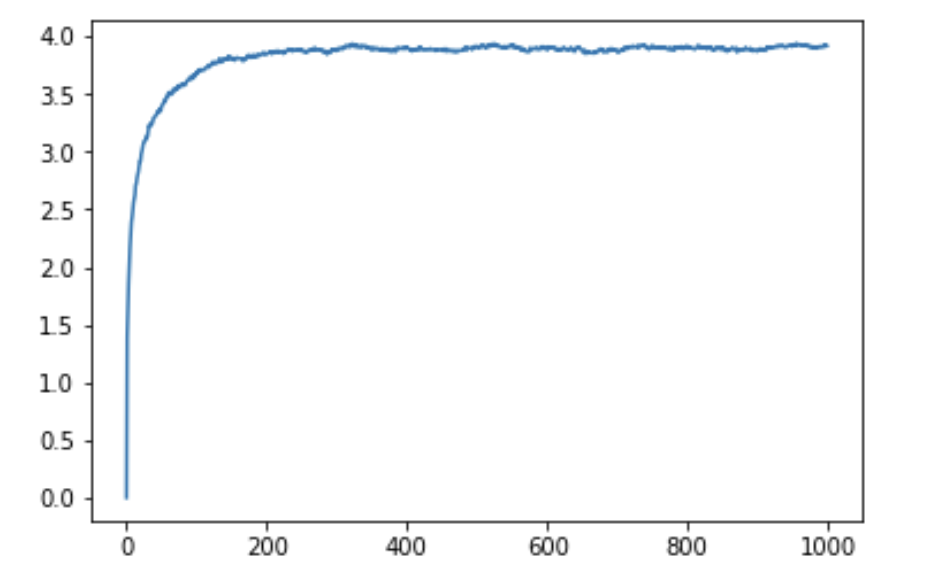
\includegraphics{rmsd}
  \caption{RMSD of 2 ns simulation.}
  \label{f1}
\end{figure}

\begin{figure}
  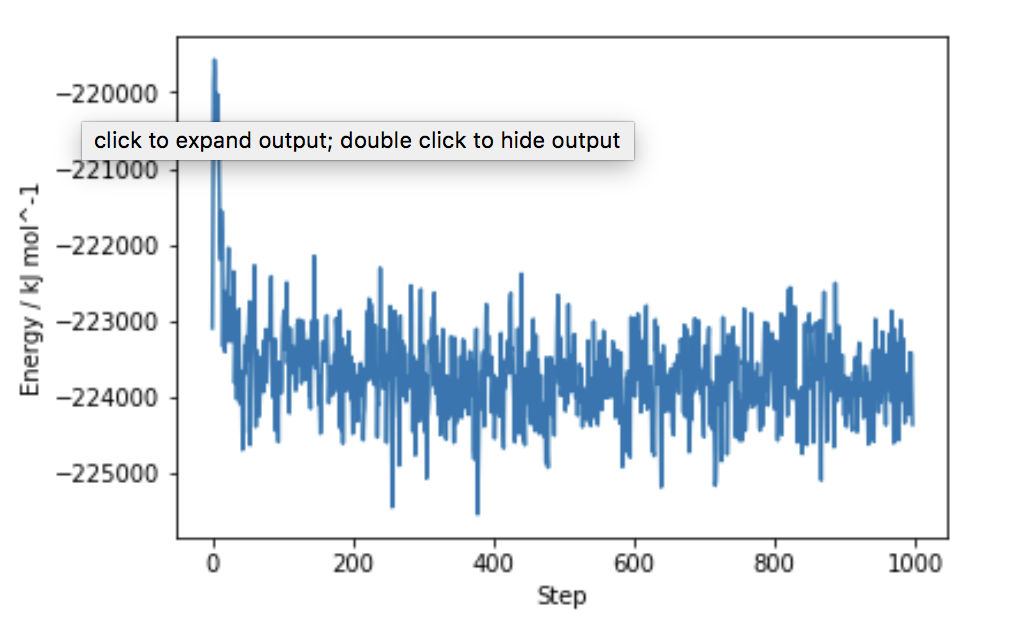
\includegraphics{energy_fluc}
  \caption{Energy fluctuation.}
  \label{f1}
\end{figure}

\begin{figure}
  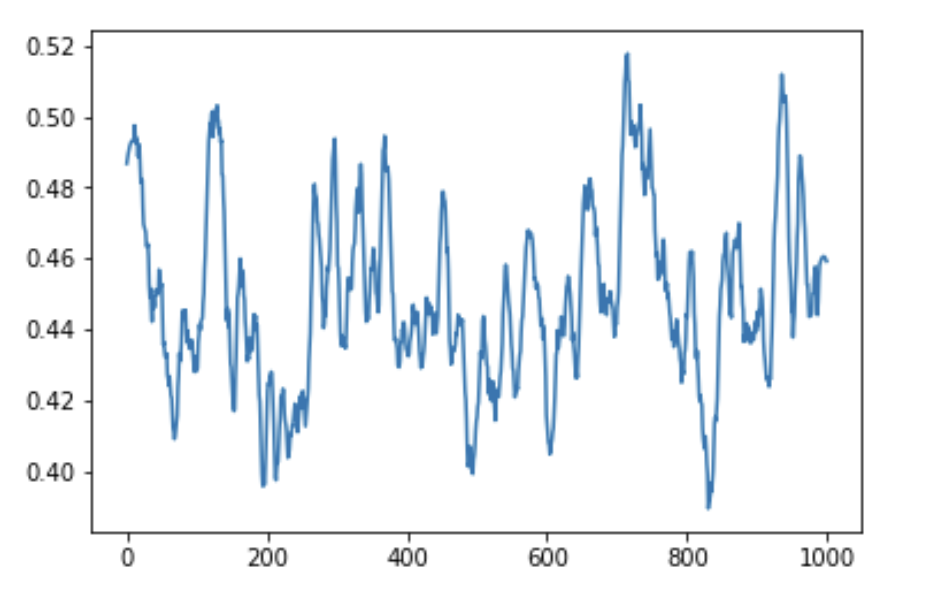
\includegraphics{basepair_distance}
  \caption{Basepair distance during simulation.}
  \label{f1}
\end{figure}


\end{document}
